\chapter{Introduction}\label{chap:key:1}
\section{Heritage speakers and their languages}\label{sec:key:1.1}

The terms \textit{heritage language} and \textit{heritage speaker} entered the field of linguistics several decades ago and soon developed into a distinct subfield within bilingualism research. Although the underlying concept has existed for as long as language contact itself, increased migration, especially to Western countries, brought new attention to it.

The concept first gained prominence in the United States, and over the past two decades, interest in heritage languages has steadily grown across Europe as well. As a result, researchers have made various efforts to define what exactly constitutes a heritage language and a heritage speaker.

One of the most widely accepted definitions comes from \citet[156]{Rothman2009}:

 “A language qualifies as a heritage language if it is a language spoken at home or otherwise readily available to young children, and crucially this language is not a dominant language of the larger (national) society […] the heritage language is acquired on the basis of an interaction with naturalistic input and whatever in-born linguistic mechanisms are at play in any instance of child language acquisition. Differently [from monolingual acquisition], there is the possibility that quantitative and qualitative differences in heritage language input, influence of the societal majority language and differences in literacy and formal education can result in what on the surface seems to be arrested development of the heritage language or attrition in adult bilingual knowledge.”

Crucially, heritage speakers are exposed to at least two languages from childhood. Typically, they encounter their heritage language from birth, which serves as their first language (L1), and they become immersed in the majority language of their society when they start attending kindergarten or school. They are also passively exposed to the majority language from birth, as it is the primary language of their environment. In some cases, speakers acquire both their heritage and majority languages simultaneously in the family. Additionally, there are instances where heritage speakers may have two heritage languages. A common scenario is when parents have different L1s: for instance, a family living in Germany where one parent speaks Spanish and the other French, so that the child acquires both languages from birth alongside German as the societal majority language. Another possibility is parents who are, for instance, Kurmanji speakers from Turkey and live in Germany, who communicate with their children in Kurmanji and Turkish. Although the parents’ L1 is Kurmanji, due to factors such as social prestige, education, or community use, they might decide to transmit both Kurmanji and Turkish as second languages (L2s) to their children. As a result, the children acquire Kurmanji and Turkish as heritage languages while also learning German as the majority language of their society.

Typically, upon entering educational institutions, the majority language of society becomes the dominant language for children and the one in which they feel most comfortable, especially in formal settings \citep{WieseEtAl2022}. While heritage speakers often continue to use their heritage language with family and friends, they frequently experience a decline in fluency due to limited or no formal exposure to that language. \citet{Matras2020} emphasizes that the level of support provided to heritage languages through media, educational institutions, and community organizations, as well as the degree of interaction and cultural exchange with the country of origin or other diaspora communities, plays a crucial role in determining the extent to which these languages can be preserved and transmitted to future generations. Furthermore, when proficiency in a particular heritage language is recognized as a valuable asset in the job market, the motivation to develop and maintain skills in that language is further enhanced.

Since the emergence of heritage language research, scholars have been working to understand the unique linguistic profiles of heritage speakers. Research has shown that the competence and performance outcomes of heritage speakers fall along a wide continuum of variability, which underpins what is referred to as the Heritage Bilingual Paradox (HBP) \citep{SchmidEtAl2019}. However, factors contributing to this variability remain a topic of ongoing debate. Recent research has aimed to model heritage language grammars, not only to explain this variability but also to enhance our understanding of linguistic competence and performance and its development in bilingual contexts.

To date, several partially overlapping proposals have been debated in the literature regarding the factors that likely contribute to the variability observed in heritage speaker grammars, as summarized by \citet{Montrul2015},  \citet{SchmidEtAl2019}, and \citet{Polinsky_Scontras_2020a, PolinskyScontras2020b}. First and probably the most obvious factor is cross-linguistic influence (CLI) -- effect of a speaker’s knowledge of one language on their knowledge or use of another \citet{jarvis_crosslinguistic_2008}. In heritage speakers, CLI most commonly occurs when features of the dominant language influence the heritage language; however, influence can also be bidirectional, depending on relative proficiency, exposure, and usage of both languages \citet{pavlenko_bidirectional_2002}. Research on heritage languages has demonstrated such CLI in lexical patterns (\citealt{DogruozBackus2009}, \citealt{Treffers-dallerEtAl2016}, \citealt{KopotevEtAl2024}), as well as in grammatical structures and constructions from one language to another (\citealt{Montrul2010}, \citealt{MontrulIonin2012}, \citealt{Van2019}).

However, the variability observed in heritage language grammars cannot be attributed to CLI alone. Another widely discussed explanation is attrition, the idea that heritage speakers may have initially acquired a particular linguistic feature or structure, but later experienced partial or complete loss of their ability in that domain. A number of studies have provided evidence for attrition, documenting the gradual loss of linguistic abilities in heritage speakers over the course of early development (e.g., \citealt{Anderson1999}, \citealt{Schmid2011}, \citealt{Silva-corvalan2014}, \citealt{Flores2015}), as well as a correlation between attrition and the length of residence in a majority-language country (\citealt{KimKim2022}). Other research has highlighted differences between child and adult heritage speakers, further supporting the role of attrition in shaping heritage language outcomes (e.g., \citealt{Montrul2015}, \citealt{Polinsky2011, Polinsky2018}).

Another proposal focuses on the different acquisition conditions experienced by heritage speakers. It highlights that bilingually raised children often shift their dominant language from the heritage language to the majority language of the society around the time they enter formal schooling. As a result of this shift, the heritage language receives significantly reduced input, which can lead to incomplete acquisition \citep{Polinsky1997, ravid_word_2005, Montrul2002, Montrul2006}.

However, some researchers argue that the term “incomplete acquisition” is problematic (\citealt{pascual_y_cabo_illogical_2012}, \citealt{PutnamSanchez2013}). This term suggests that the ultimate attainment in language acquisition is possible, based on the notions that there is a final stage in the acquisition of monolingual grammars and that this stage varies minimally across speakers (\citealt{PutnamSanchez2013}). While one could contend that a final stage of monolingual language acquisition exists, research indicates significant inter-individual variation in monolingual grammars as well (e.g., \citealt{ShadrovaEtAl2021}). This variation arises because the acquisition of a language, even when it is the only language spoken by an individual, is influenced by various factors, such as socioeconomic status and educational background.

Additionally, \citet{pascual_y_cabo_illogical_2012} highlight that heritage speakers receive different input compared to monolinguals, as their language exposure is often shaped by language attrition in the first generation or by language contact. Consequently, the acquisition of a heritage language by heritage speakers is not incomplete, rather, it is just different. \citet{AustinEtAl2013}, further notes that while increased exposure to the dominant language of society may impede L1 acquisition, it does not necessarily result in the incomplete acquisition of certain L1 features. Instead, this phenomenon can be understood as a different trajectory toward complete acquisition, accounting for the unique characteristics of bilingualism. Hence, \citet{PutnamSanchez2013} propose to refer to this developmental path as divergent attainment in heritage speakers.

That said, it is important to recognize that the various proposals that explain differences in heritage speaker competence and performance, such as CLI, attrition, and divergent attainment, are not mutually exclusive but rather complementary. The challenge lies in predicting when each of these processes will arise, in which linguistic domains, and across which language constellations.

Although these accounts provide a broad framework and incorporate multiple explanatory factors, they often give limited attention to the role of internal dynamics in a language, such as the variation and variability inherent to monolingual speakers’ language, which can be amplified or maintained by heritage speakers (\citealt{FloresRinke2020}). Building on this, an internal factor that is particularly relevant is register. While heritage language research often acknowledges the diglossic nature of bilingual speakers’ repertoires -- where different languages are used depending on the domain or situation (\citealt[323-324]{Polinsky2018}) -- variation across registers within the heritage language itself has received comparatively little attention. \citet{WieseEtAl2022} show that noncanonical linguistic phenomena—features that deviate from standard norms—occur not only in heritage language use but also in the informal speech of monolingual speakers, suggesting that some patterns observed in heritage grammars may not result solely from CLI, attrition, or incomplete acquisition, but instead reflect register-specific distributions that are also attested in monolingual speakers. Thus, in the present study, register will be analyzed as one of the factors influencing heritage language outcomes.

Another widely discussed issue in heritage language research is the question of comparability. To date, heritage speakers are most often compared to monolingual speakers residing in the country of origin of the heritage speakers’ parents or grandparents (\citealt{RothmanEtAl2023}, \citealt{alexiadou_methodological_2025}). These monolinguals are typically treated as the benchmark for comparison. However, as the preceding discussion makes clear, monolinguals follow a different developmental trajectory in language acquisition, which raises questions about the validity of such comparisons.

Less frequently, studies have compared heritage adults and heritage children (\citealt{Polinsky2011, Polinsky2018}), heritage speakers and so-called “returnees” (\citealt{Treffers-dallerEtAl2007}, \citealt{FloresEtAl2022}), heritage speakers and L2 learners (\citealt{MontrulEtAl2008}, \citealt{Perez-cortes2016}), or heritage and first-generation speakers (\citealt{CoskunMontrul2022, CoskunMontrul2025}). Even less common are comparisons between heritage speakers and bilingual speakers residing in the country of origin of the heritage speakers’ parents or grandparents. In the context of this study, this concerns in particular Turkish-Kurdish bilinguals in Turkey, who acquire both languages from early childhood and grow up in a setting where Turkish functions as the majority language. These speakers, like heritage speakers, are early bilinguals; however, unlike Turkish heritage speakers in Germany, Turkish remains the majority and dominant language in their environment. Such comparisons shift the focus away from a simple monolingual-bilingual distinction towards the societal status of the language, in particular whether it functions as a majority or heritage language in a given context. That said, given that the majority of speakers worldwide are multilingual \citep{Grosjean2001}, it is essential not to rely solely on these groups as benchmarks for comparison, instead, they should be considered alongside other bilingual groups in analyses.

Finally, an important aspect that is receiving increasing attention in heritage language research is the range of languages and the countries of the speakers being studied. \citet{FridmanÖzsoy2024} emphasize that heritage language research lacks linguistic diversity. Their analysis of over 1,000 articles from Scopus reveals a clear bias toward certain languages within the field. The figure below illustrates the top ten pairs of heritage and majority languages examined in the research.

\begin{figure}
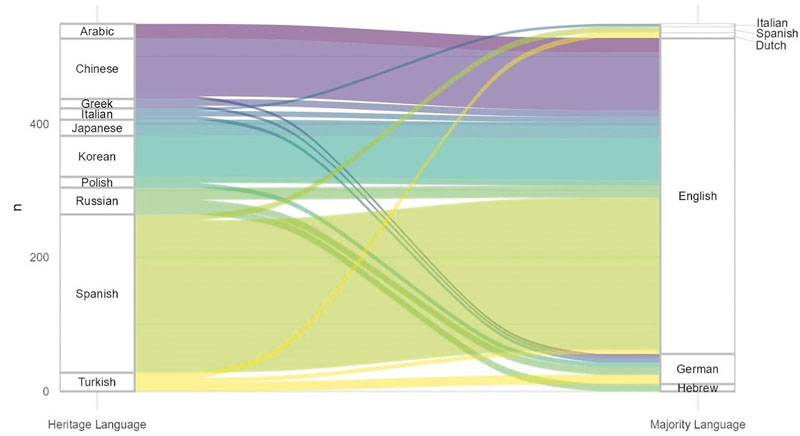
\includegraphics[width=\textwidth]{figures/iefremenko-img001.jpg}
\caption{\label{fig:key:1}: Top 10 subfields in HL research based on a literature survey (\citealt{FridmanÖzsoy2024})}
\end{figure}

\figref{fig:key:1} demonstrates that English is the most common majority language, with German coming in a distant second. Spanish is the most widely studied heritage language, followed by Chinese and Korean, all of which are primarily researched in the context of majority English. Other investigated heritage languages include Arabic, Greek, Italian, Japanese, Polish, Russian, and Turkish.

\section{Objectives and scope of this study}\label{sec:key:1.2}

In light of the current debates in heritage language research, this study aims to:

\begin{enumerate}
    \item Contribute to understanding and modeling heritage language grammars by considering the aforementioned proposals and examining factors such as CLI and internal dynamics in the languages, particularly the role of register.
    \item Expand the comparative framework by including bilingual majority speakers, thereby shifting the focus from a simple mono- versus bilingualism dichotomy to an analysis of the status of the languages under investigation (heritage vs. majority).
    \item Focus on the relatively frequently studied heritage language Turkish and the largely unexplored Kurmanji Kurdish within the context of the majority German and majority Turkish languages.
\end{enumerate}

To address these aims, the study examines two languages—Turkish and Kurmanji Kurdish—across four speaker populations: Turkish heritage speakers in Germany, Turkish-Kurmanji heritage speakers in Germany, Turkish-Kurmanji bilinguals in Turkey, and Turkish monolinguals in Turkey.

Let us discuss the objectives in reverse, beginning with the third. This study concentrates on two languages, Turkish and Kurmanji. While Turkish has been the subject of heritage language research—although primarily in the German context—Kurmanji Kurdish remains largely overlooked. This study investigates Kurmanji in two countries, Germany and Turkey. While Kurmanji is clearly recognized as a heritage language in the German context, its classification as such in Turkey is less common.

According to \citegen{Rothman2009} definition, a heritage language is one that is acquired early in life in a naturalistic setting but is not the dominant language of the wider society. Although this definition applies to many language constellations and minoritized languages around the world, as shown in the figure above, most heritage language research focuses on immigrant contexts in the Global North. Nevertheless, minoritized languages like Kurmanji Kurdish in Turkey exhibit the same characteristics described in Rothman’s definition of a heritage language. As will be discussed in Chapter \ref{chap:key:2}, Kurmanji is primarily acquired at home, while Turkish functions as the dominant language of the society. Consequently, Kurmanji speakers often have very limited exposure to their heritage language and lack opportunities for formal acquisition in educational settings (\citealt{BulutOpengin2018}). For this reason, Kurmanji in Turkey is classified as a heritage language in this study.

Nevertheless, several important differences must be considered. Unlike “classic” heritage languages, minoritized languages typically lack a corresponding majority variety, and their speakers are often bilingual or even multilingual. This makes comparisons feasible only among different groups of heritage speakers, whether based on age or between those who have different majority languages in contact. Additionally, minoritized languages frequently lack standardization and may not exhibit a wide range of registers \citep[323-324]{Polinsky2018}.

Furthermore, the contact between minoritized languages and the majority language in a given society is often longer and more intense than that of “classic” heritage languages in the Global North. In the field of language contact research, the intensity of contact—defined by the number of speakers in the community and the duration of contact—is considered a crucial social factor for predicting contact-induced language change: the more intense the contact, the greater the likelihood of structural changes (\citealt{ThomasonKaufman1988}). Thus, these differences will be taken into account in subsequent discussions throughout the study.

The second objective of this study is to broaden the comparative framework by incorporating bilingual majority speakers in Turkey whose first language is Kurmanji and whose second language is Turkish. This approach allows us to analyze two groups where Turkish serves as the majority language: monolingually and bilingually raised speakers. By incorporating these groups, the focus shifts from bilingualism itself to the status of the language being studied, whether it is a heritage or majority language. Furthermore, there are only a handful of studies on the Turkish spoken by Kurmanji-Turkish bilinguals in Turkey, and this study aims to establish a foundation for future research in this area.

Finally, the last objective of this study is to contribute to a better understanding of heritage language grammars and the factors that may account for the wide range of competences and performances observed among heritage speakers. This includes examining CLI influence and internal linguistic dynamics, with the focus on the role of register.

It is important to note that research on the factors shaping outcomes of languages in contact did not originate in heritage language studies, but in the broader field of contact linguistics. Within this field, linguists often differentiate between externally and internally motivated change \citep{Hickey2020}. Externally motivated changes, often referred to as instances of CLI, arise from contact with another language and result into the transfer of lexical or structural features from a dominant language (\citealt{jarvis_crosslinguistic_2008}, \citealt{ThomasonKaufman1988}, \citealt{Matras2009, Matras2020}). Internally motivated changes, in contrast, emerge from the language's own dynamics, including processes such as variation, generational transmission, and youth language (\citealt{Labov1994, Labov2001, Labov2010}, \citealt{PoplackLevey2010}, \citealt{Tagliamonte2016}).

The phenomenon of CLI is described using a variety of terms. It is often understood as the transfer of structures or forms from one language to another, and is commonly referred to as borrowing. Linguists typically distinguish between two main types of borrowing. The first involves the direct adoption of specific linguistic items, such as words or fixed expressions, from one language into another, and has been variously labeled “importation” \citep{Haugen1950}, “selective copying” \citep{Johanson2002}, or “matter replication” \citep{Matras2020}. The second type involves the borrowing of underlying grammatical and structural patterns or constructions, rather than just isolated lexical items. \citet{Haugen1950} refers to this as a “calque”, \citet{Johanson2002} as “global copying”, and \citet{Matras2020} as “pattern replication”. A related concept is “convergence” \citep{Weirich1953}, which can be understood as a mutual process or affect only one of the languages in contact \citep{Matras2020}. Throughout this study, the term \textit{cross-linguistic influence} will refer broadly to all types of contact-induced changes discussed above.

Understanding how language changes requires examining the underlying linguistic mechanisms. From the perspective of the usage-based approach, language is not simply a system of abstract rules but a dynamic inventory of patterns and constructions that emerge from actual use (\citealt{Bybee2010}, \citealt{langacker_foundations_1987}, \citealt{Dabrowska2019}). In this framework, constructions are grammatical units of varying size and complexity in which specific structural patterns are associated with particular functions or meanings. Constructions lie on a continuum from fully specific lexicalized units, such as idioms (kick the bucket) or prefabricated expressions (I don’t know), to highly schematic patterns, such as imperative forms or generalized argument structures (\citealt{langacker_foundations_1987}, \citealt{Goldberg2006}, \citealt{Nicolai2014}). Partially schematic constructions occupy the intermediate space, with some elements fixed and others open for lexical insertion. Structural change can therefore be understood as the cumulative outcome of how these constructions are stored, accessed, and generalized by speakers.

Frequency of use is a crucial factor in language change. Highly entrenched constructions are more resistant to modification and tend to be preserved over time, whereas less frequent or less entrenched constructions are more vulnerable to change or replacement (\citealt{langacker_foundations_1987}, \citealt{Tomasello2010}, \citealt{HakimovBackus2021}). In multilingual environments, speakers often generalize across their language repertoire, adopting structures present in multiple languages and producing shared constructions more frequently when the languages involved are similar and contact is prolonged (\citealt{Ansaldo2009}, \citealt{Matras2020}).

The usage-based approach also emphasizes the role of individual speakers in driving change. Language change is seen as the cumulative effect of repeated choices made during interaction: as constructions are repeatedly used by more speakers, they become more entrenched and can eventually lead to conventionalized patterns at the community level (\citealt{Nicolai2014}, \citealt{Bybee2006}). The propagation of innovations is gradual, and not all new constructions become conventionalized, the likelihood of adoption depends on factors such as directionality of bilingualism and social pressure to adhere to established norms \citep{Matras2020}.

Furthermore, structural and usage-based perspectives can be complemented by consideration of social factors, which have consistently been highlighted as primary determinants of language change. \citet{ThomasonKaufman1988} argue that while linguistic factors such as typological constraints can shape possible outcomes, it is the sociolinguistic context of the speakers that largely governs what changes occur and to what extent. Key social factors include imperfect learning, arising from incomplete acquisition of a target language, speakers’ attitudes toward the languages and the contact situation, and the intensity of contact, determined by both the number of speakers involved and the duration of the language contact. Intensity of contact influences the depth of linguistic change: in casual contact situations, borrowing is typically limited to content words, whereas in more intense contact situations, structural features—including word order, clause-combining strategies, and inflectional morphology—are more likely to be affected \citep{Thomason2022}.

Other influential factors include language dominance and prestige, the degree of bilingualism, and institutional support such as literacy, schooling, and media exposure (\citealt{Johanson2002}, \citealt{Matras2020}), the language user’s level of proficiency in the source language, as well as the frequency and recency of use of the post-L1 source language and its degree of similarity to the recipient language (\citealt{jarvis_crosslinguistic_2008}). Together, these factors shape both the features that are transferred and the direction of influence.

As noted earlier, CLI in heritage language research has received considerable attention. While contact between the heritage and the majority languages is undoubtedly ubiquitous, changes in the heritage language cannot always be attributed to CLI. Thus, \citet{FloresRinke2020} highlight another factor that should be taken into consideration and is often overlooked in the studies, namely language-internal phenomena of variation and variability. Even in monolingual varieties, language change can take place due to internal dynamics, including processes such as variation, analogical restructuring, generational transmission, and innovations in youth speech communities (\citealt{Labov1994, Labov2001, Labov2010}, \citealt{PoplackLevey2010}, \citealt{Tagliamonte2016}). \citet{FloresRinke2020} argue that heritage speakers may boost and further develop tendencies of language (internal) evolution inherent to variable phenomena. Furthermore, they may also retain variation that is typical of non-standard registers, because they are mainly exposed to colloquial input.

Building on these insights, this study focuses on the role of register in heritage language outcomes—a factor that has received relatively little systematic attention in heritage language research. In this study, register is defined as “those aspects of socially recurring intra-individual variation that are influenced by situational and functional settings” \citep[3]{ludeling_register_2022}. This means that patterns of variation are socially recurrent—speakers tend to adjust their language use in similar ways across comparable contexts. At the same time, this variation is fundamentally intra-individual: it is the same speaker who systematically varies their linguistic choices depending on the communicative setting. In this sense, register captures how socially structured patterns of language use are realized within individuals across different contexts. \citet{HallidayEtAl1964} and \citet{Halliday1989} distinguish between three components that serve as a model for understanding the situational-functional context of register: field, tenor, and mode. In this framework, the field relates to the subject matter or topic of discourse, the tenor involves social roles, relationships, and power dynamics among participants, while the mode refers to the channel of communication (spoken or written). \citet{Wiese2021} further highlights that such situational characteristics identify communicative situations.

Communicative situations will play a pivotal role in the methodology of the current study. In this context, the two defining parameters of communicative situations are formality and mode, each featuring two levels: informal versus formal and spoken versus written. The specific examples of the communicative situations used in the current study will be given in the Chapter \ref{chap:key:4}, Methodology.

From the above-given discussion on registers and communicative situations, it is evident that linguistic features constitute registers while situational characteristics define communicative situations. Consequently, register knowledge is the knowledge of the alignment of particular linguistic forms and structures with certain situations \citep{PescumaEtAl2023}. For instance, speakers may choose different structures depending on an interlocutor, the formality of the situation, the mode, the purpose of the conversation, etc.

Register can play an important role in understanding heritage speakers’ languages. As discussed at the beginning of this chapter, heritage speakers usually acquire their heritage language at home and often have limited exposure to formal registers in their heritage language. Many studies investigating heritage languages rely on data collected in informal settings, which is sometimes implicitly compared to the norms of the standard language of majority speakers. This approach can put heritage speakers at a disadvantage, as it overlooks the role of register in shaping language use.

\citet{WieseEtAl2022} emphasize the importance of selecting an appropriate baseline for comparison. Their findings show that noncanonical linguistic phenomena—features that deviate from standard norms—do occur in heritage language use, but crucially, they are also frequently observed in the informal speech of monolingually raised speakers of the same language.

Incorporating data elicited across different communicative situations into heritage language research is essential for ensuring fairer and more accurate comparisons between heritage and majority speakers. By accounting for register in both data collection and analysis, researchers can better isolate whether observed differences are truly due to heritage language development or simply reflect informal, nonstandard usage. Moreover, examining the informal speech of majority language speakers provides valuable insights into broader linguistic trends, including whether certain features associated with heritage speakers might actually reflect ongoing changes within the majority language itself.

The investigated linguistic phenomenon chosen for the study is word order, specifically the post-predicate position in Turkish and Kurmanji Kurdish. The rationale for concentrating on this position is that the languages under investigation here, Turkish, Kurmanji, and German, are SOV languages, yet they employ the post-predicate position to a different extent. Moreover, the employment of this position is determined by different factors in each language: information structure in Turkish (\citealt{Erguvanli1984}, \citealt{Erku1983}, \citealt{Issever2003}), predicate semantics in Kurmanji (\citealt{Gundogdu2019}, \citealt{Haig2018, Haig2020}), and syntactic structure in German (\citealt{Frey2015}, \citealt{Muller2023}).

Despite the differences across languages, several overlapping factors influence the use of the post-predicate position. \citet{Asadpour2021}, for instance, shows that in Mukri Kurdish spoken in Iran, information structure—alongside predicate semantics—affects word order. If similar patterns are found in Kurmanji Kurdish spoken in Turkey, this would suggest that information structure plays a shared role in both Kurmanji and Turkish. Additionally, factors such as mode and formality influence the use of post-predicate constituents in Turkish and German, where they are more common in spoken than written language, and in informal rather than formal situations (\citealt{Schroeder1995, Schroeder2002}, \citealt{Tsehaye2023}). Although the effect of mode and formality are underexplored in Kurmanji, evidence from related languages like Persian suggests they may be relevant (\citealt{Frommer1981, Haig_post-predicate_EtAl2024-1}). Thus, such differences and similarities create opportunities for interesting developments in these languages, driven by language contact.

The manuscript is organized as follows: Chapter \ref{chap:key:2} introduces the communities investigated in this study. Chapter \ref{chap:key:3} discusses word order in Turkish, Kurmanji, and German, providing an overview of previous research on the post-predicate position in these languages. After establishing the theoretical background, Chapter \ref{chap:key:4} outlines the methodology, participants, corpus, and details of the analysis process. Chapters \ref{chap:key:5} and \ref{chap:key:6} present the results for Turkish and Kurmanji, respectively. Chapter \ref{chap:key:7} addresses the research objectives, examines CLI, internal dynamics, and the role of register, and discusses the study’s limitations. Chapter \ref{chap:key:8} offers a concluding overview.

